\chapter{静电场}
\section{作业习题}
\subsection*{一、填空题}
\begin{enumerate}
    \item 边长为$a$的正方形的四个顶点上放置如图所示 \ref{fig:46} 的点电荷, 则中心$o$处场强为\nl.
    \begin{figure}[H]
        \centering
        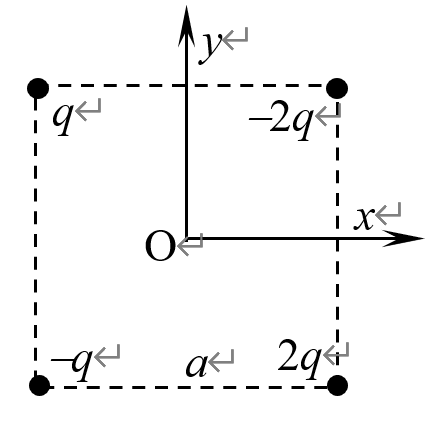
\includegraphics[width=0.15\textheight]{fig46}
        \caption{如图.}\label{fig:46}
    \end{figure}
    \item 在点电荷系的电场中, 任一点的电场强度等于\nl, 这称为电场强度叠加原理.
    \item 正方形的两对角上, 各置电荷$Q$, 在其余两对角上各置电荷$q$, 若$Q$所受合力为零,则$Q$与$q$的大小关系为$\nl$.
    \item   如图所示 \ref{fig:49}, 真空中有两个点电荷, 带电量分别为$Q$和$-Q$, 相距$2R$。若以负电荷
    所在处$O$点为中心, 以$R$为半径作高斯球面$S$, 则通过该球面的电场强度通量$\varphi_e=\nl$. 
    \begin{figure}[H]
        \centering
        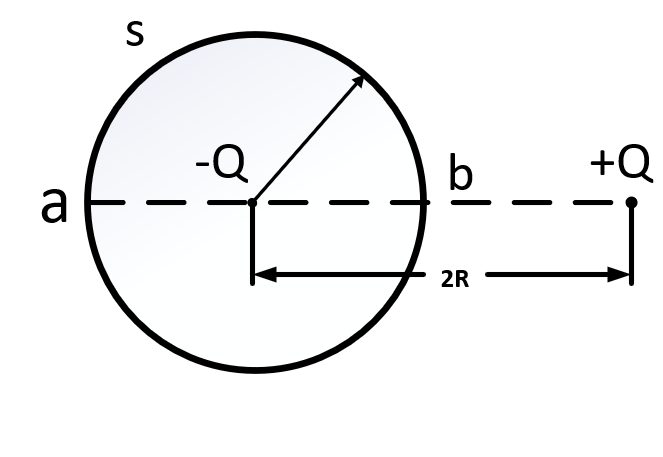
\includegraphics[width=0.15\textheight]{fig49}
        \caption{如图.}\label{fig:49}
    \end{figure}
    \item 如图所示\ref{fig:50}, 在场强为$E$的均匀电场中取一半球面, 其半径为$r$, 电场强度的方向与半球面的对称轴平行. 则通过这个半球面的电通量$\varphi_e=\nl$.
    \begin{figure}[H]
        \centering
        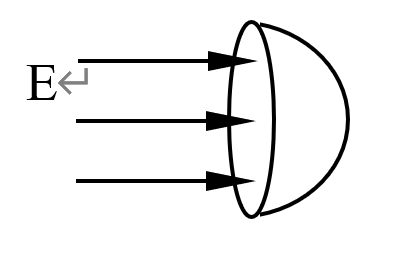
\includegraphics[width=0.15\textheight]{fig50}
        \caption{如图.}\label{fig:50}
    \end{figure}
    \item 一点电荷$q$位于一位立方体中心, 立方体边长为$a$, 则通过立方体每个表面的$\vec{E}$的通量\nl;若把这电荷移到立方体的一个顶角上, 这时通过电荷所在顶角的三个面$\vec{E}$的通量是\nl, 通过立方体另外三个面的$\vec{E}$的通量是\nl.
    \item 一均匀静电场, 场强$\vec{E}=(400\vec{i}+600\vec{j})v\cdot m^{-1}$, 则点$a(3, 2)$和点$b(1, 0)$之间的电势差$U_{ab}=\nl$.
    \item 如图所示\ref{fig:52}, 半径为$R$的均匀带电球面, 总电荷为$Q$, 设无穷远处的电势为零, 则球内距离球心为$r$的$P$点处的电势$U=\nl$. 
    \begin{figure}[H]
        \centering
        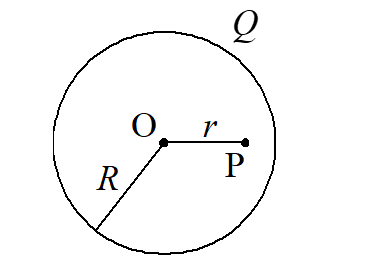
\includegraphics[width=0.15\textheight]{fig52}
        \caption{如图.}\label{fig:52}
    \end{figure}
    \item 一“无限长”均匀带电直线沿$Z$轴放置, 线外某区域的电势表达式为$U=A\mathrm{ln}(x2+y2)$, 式中$A$为常数, 该区域电场强度的两个分量为: $E_x$=\nl, $E_y$=\nl.
\end{enumerate}
\subsection*{二、选择题}
\begin{enumerate}
    \item 如图所示 \ref{fig:47}, 一电偶极子, 正点电荷在坐标$(a,0)$处, 负点电荷在坐标$(-a,0)$处, $P$点是$x$轴上的一点, 坐标为$(x,0)$. 当$x>>a$时, 该点场强的大小为(\hspace{1pc})
    \fourch{$\frac{q}{4\pi\varepsilon_0x}$;}{$\frac{q}{4\pi\varepsilon_0x^2}$;}{$\frac{qa}{2\pi\varepsilon_0x^3}$}{$\frac{qa}{\pi\varepsilon_0x^3}$.}
    \begin{figure}[H]
        \centering
        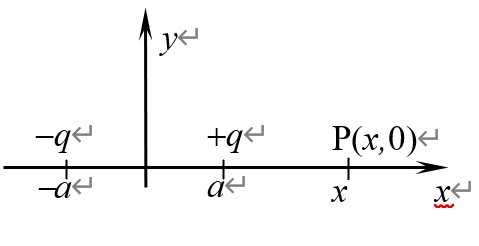
\includegraphics[width=0.15\textheight]{fig47}
        \caption{如图.}\label{fig:47}
    \end{figure}
    \item 真空中面积为$S$, 间距$d$的两平行板$S>>d_2$, 均匀带等量异号电荷+q和-q, 忽略边缘效应, 则两板间相互作用力的大小是(\hspace{1pc}).
    \twoch{$\frac{q^2}{(4\pi\varepsilon_0d^2)}$; }{$\frac{q^2}{(\varepsilon_0 s)}$;}{$\frac{q^2}{(2\varepsilon_0s)}$;}{$\frac{q^2}{(2\pi\varepsilon_0d^2)}$.}
    \item  下列哪一种说法正确 (\hspace{1pc})
    \onech{电场线上任意一点的切线方向, 代表这点的电场强度的方向;}{在某一点电荷附近的任一点, 若没放试验电荷, 则这点的电场强度为零;}{若把质量为$m$的点电荷$q$放在一电场中, 由静止状态释放, 电荷一定沿电场线运动;}{电荷在电场中某点受到的电场力很大, 该点的电场强度一定很大.}
    \item 关于高斯定理的理解有下面几种说法, 其中正确的是(\hspace{1pc})
    \onech{如果高斯面上$\vec{E}$处处为零, 则该面内必无电荷;}{如果高斯面内无电荷, 则高斯面上$\vec{E}$处处为零;}{如果高斯面上$\vec{e}$处处不为零, 则高斯面内必有电荷;}{如果高斯面内有净电荷, 则通过高斯面的电场强度通量必不为零.}
    \item 下述带电体系的场强分布可能用高斯定理来计算的是(\hspace{1pc})
    \twoch{均匀带电圆板}{有限长均匀带电棒}{电偶极子}{带电介质球(电荷体密度是离球心距离$r$的函数)}
    \item 已知某电场的电场线分布情况如图所示\ref{fig:53}. 现观察到一负电荷从$M$点移到$N$点. 有人根据这个图作出下列几点结论, 其中正确的是(\hspace{1pc})
    \twoch{电场强度$E_M$<$E_N$}{电势$U_M$<$U_N$}{电势能$W_M$<$W_N$}{电场力的功$A>0$}
    \begin{figure}[H]
        \centering
        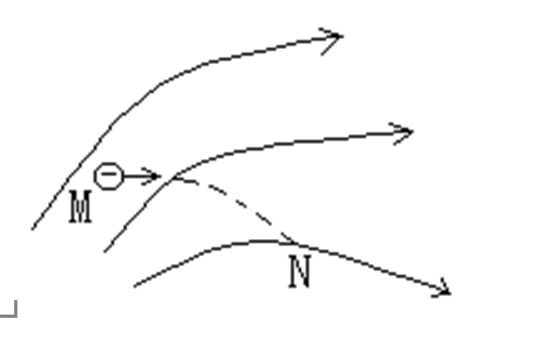
\includegraphics[width=0.15\textheight]{fig53}
        \caption{如图.}\label{fig:53}
    \end{figure}
    \item 如图所示\ref{fig:54}, 下面表述中正确的是(\hspace{1pc})
    \twoch{$E_A$>$E_B$>$E_C$, $U_A$>$U_B$>$U_C$}{$E_A$<$E_B$<$E_C$, $U_A$>$U_B$>$U_C$}{$E_A$>$E_B$>$E_C$, $U_A$<$U_B$<$U_C$}{$E_A$<$E_B$<$E_C$, $U_A$<$U_B$<$U_C$}
    \begin{figure}[H]
        \centering
        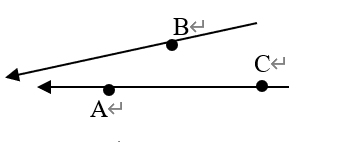
\includegraphics[width=0.15\textheight]{fig54}
        \caption{如图.}\label{fig:54}
    \end{figure}
    \item 下列关于静电场的说法中, 正确的是(\hspace{1pc})
    \onech{电势高的地方场强就大}{带正电的物体电势一定是正的}{场强为零的地方电势一定为零}{电场线与等势面一定处处正交}
\end{enumerate}
\subsection*{三、计算题}
\begin{enumerate}
    \item 如图 \ref{fig:48}, 内半径为$R_1$, 外半径为$R_2$的环形薄板均匀带电, 电荷面密度为$\sigma$, 求: 中垂线上任一$P$点的场强及环心处0点的场强.
    \begin{figure}[H]
        \centering
        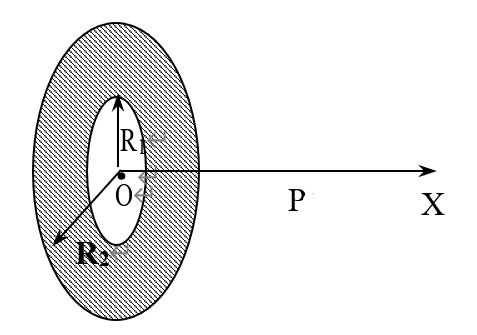
\includegraphics[width=0.15\textheight]{fig48}
        \caption{如图.}\label{fig:48}
    \end{figure}
    \item 如图 \ref{fig:51}, 无限长均匀带电圆柱体,电荷体密度为$\rho$, 半径为$R$, 求柱体内外的场强分布.
    \begin{figure}[H]
        \centering
        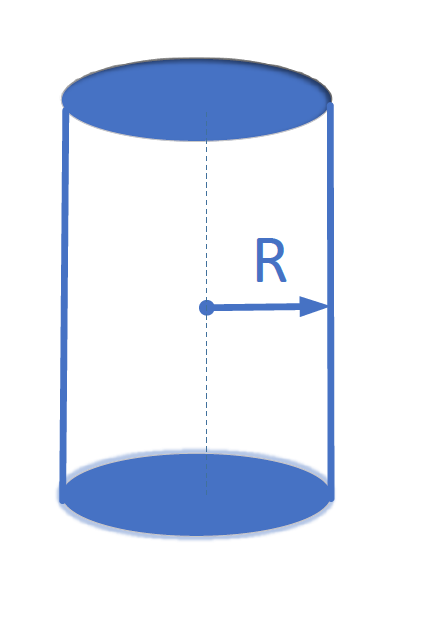
\includegraphics[width=0.15\textheight]{fig51}
        \caption{如图.}\label{fig:51}
    \end{figure}

    \item 如图 \ref{fig:55}, 球壳的内半径为$a$, 外半径为$b$, 壳体内均匀带电, 电荷体密度为$\rho$, 求: 空间的场强和电势分布.
    \begin{figure}[H]
        \centering
        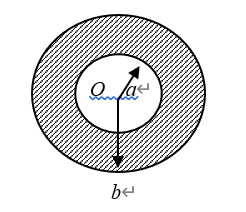
\includegraphics[width=0.15\textheight]{fig55}
        \caption{如图.}\label{fig:55}
    \end{figure}
\end{enumerate}